% Autor: Simon May
% Datum: 2017-10-05
% Diese Datei bietet ein minimalistisches Grundgerüst für ein LaTeX-Dokument,
% z.B. für die Bearbeitung der Aufgaben.
\documentclass[
	% Papierformat
	a4paper,
	% Schriftgröße (beliebige Größen mit „fontsize=Xpt“)
	12pt,
	% Schreibt die Papiergröße korrekt ins Ausgabedokument
	pagesize,
	% Sprache für z.B. Babel
	ngerman
]{scrartcl}

% Achtung: Die Reihenfolge der Pakete kann (leider) wichtig sein!
% Insbesondere sollten (so wie hier) babel, fontenc und inputenc (in dieser
% Reihenfolge) als Erstes und hyperref und cleveref (Reihenfolge auch hier
% beachten) als Letztes geladen werden!

% Silbentrennung etc.; Sprache wird durch Option bei \documentclass festgelegt
\usepackage{babel}
% Verwendung der Zeichentabelle T1 (Sonderzeichen etc.)
\usepackage[T1]{fontenc}
% Legt die Zeichenkodierung der Eingabedatei fest, z.B. UTF-8
\usepackage[utf8]{inputenc}
% Schriftart
\usepackage{lmodern}
% Zusätzliche Sonderzeichen
\usepackage{textcomp}

% Mathepaket (intlimits: Grenzen über/unter Integralzeichen)
\usepackage[intlimits]{amsmath}
% Ermöglicht die Nutzung von \SI{Zahl}{Einheit} u.a.
\usepackage{siunitx}
% Zum flexiblen Einbinden von Grafiken (\includegraphics)
\usepackage{graphicx}
% Abbildungen im Fließtext
\usepackage{wrapfig}
% Abbildungen nebeneinander (subfigure, subtable)
\usepackage{subcaption}
% Funktionen für Anführungszeichen
\usepackage{csquotes}
% Zitieren, Bibliographie
\usepackage{biblatex}

% Verlinkt Textstellen im PDF-Dokument
\usepackage[unicode]{hyperref}
% "Schlaue" Referenzen (nach hyperref laden!)
\usepackage{cleveref}

% siunitx: Deutsche Ausgabe, Messfehler getrennt mit ± ausgeben
\sisetup{
	locale=DE,
	separate-uncertainty
}

\begin{document}
\begin{titlepage}
	\centering
	{\scshape\LARGE Versuchsbericht zu \par}
	\vspace{1cm}
	{\scshape\huge O4 - Magneto-Optischer-Kerr-Effekt \par}
	\vspace{2.5cm}
	{\LARGE Gruppe 6 Mo\par}
	\vspace{0.5cm}
	{\large Nils Kulawiak (E-Mail: n\_kula01@wwu.de) \par}
	{\large Oliver Brune (E-Mail: o\_brun02@wwu.de) \par}
	\vfill
	durchgeführt am 11.06.2018\par
	
	\vfill
	betreut von Christoph Angrick
	{\large \today\par}
\end{titlepage}

\tableofcontents
		
\newpage

\section{Methoden und Durchführung}
In diesem Versuch wurden verschiedene Eigenschaften von Röntgenstrahlung untersucht. Hierfür wurde eine Röntgenröhre mit Kupferanode verwendet. Der schematische Aufbau einer Röntgenröhre ist in \cref{roentgen} dargestellt.

\begin{figure}[h!]
	\centering
	\includegraphics[scale = 1]{roentgen.png}
	\caption{Schematischer Aufbau einer Röntgenröhre}
	\label{roentgen}
\end{figure}

In einem Gehäuse, in dem ein Vakuum herrscht, befinden sich Kathode und Anode der Röntgenröhre. Die Kathode besteht aus einem Metalldraht, oft Wolfram, der mit einer Heizspannung zum Glühen gebracht wird. Dadurch werden Elektronen aus dem Draht herausgelöst und bilden eine Elektronenwolke um den Draht. Wenn nun eine Anodenspannung angelegt wird (in diesem Versuch meist \SI{35}{kV}), dann werden die Elektronen in Richtung der Anode beschleunigt. In diesem Versuch besteht die Anode aus Kupfer. Treffen die hochenergetischen Elektronen auf das Kupfer, werden sie durch Wechselwirkung mit den Atomen abgebremst, es entsteht Bremsstrahlung mit einem kontinuierlichen Energiespektrum. Aus diesem Spektrum stechen allerdings bestimmte Energien deutlich heraus, die öfter erzeugt werden. Das sind die Röntgenstrahlen, die entstehen, wenn ein freies Elektron ein Elektron aus der K-Schale eines Kupferatoms ionisiert. Wenn das passiert, füllt ein Elektron aus der L- oder der M-Schale den freigewordenen Platz auf. Die Energiedifferenz zwischen den beiden Schalen gibt das Elektron dann in Form von Röntgenstrahlung ab. Die Linien im Energiespektrum sind dann gerade die so erzeugten Röntgenstrahlen. Diese sind atomspezifisch, daher nennt man diese Strahlung charakteristische Röntgenstrahlung.

Die Anode steht in einem $45$°-Winkel zum Elektronenstrahl, damit die Röntgenstrahlung möglichst in Richtung der Probe gerichtet ist. Die Strahlung wird anschließend von einer Blende kollimiert, damit nur nahezu parallele Strahlen auf die Probe treffen. Die Probe ist in diesem Experiment immer einer von zwei Kristallen, an denen Bragg-Reflexion durchgeführt wird. Der eine ist ein LiF-Einkristall, der andere ein KBr-Einkristall. An diesen findet Bragg-Reflexion statt, sodass je nach Einfallswinkel immer genau eine Wellenlänge die Bragg-Bedingung erfüllt, die dann reflektiert wird und von einem Geiger-Müller-Zählrohr detektiert wird. Um das gesamte Spektrum der Röntgenstrahlung abzutasten, muss daher der Kristallwinkel und damit auch der Detektorwinkel variiert werden. Der abgefahrene Winkelbereich war bei jedem Versuchsteil unterschiedlich. Der Winkel wurde in $0,1$°-Schritten variiert, gemessen wurde in jeder Einstellung $2$ Sekunden lang.

Da beim Geiger-Müller-Zählrohr bei jedem detektierten Photon eine vollständige Gasentladung stattfindet, gibt es einen kurzen Zeitraum, in dem keine weitere Strahlung detektiert werden kann. Dieses Zeitintervall bezeichnet man als Totzeit, sie beträgt bei dem verwendeten Zählrohr etwa $\SI{90}{\micro \second}$. Um die tatsächliche Anzahl an Teilchen zu bestimmen, die auftreten, wird \cref{eq:korr} verwendet. Dabei ist $\tau$ die Totzeit $N$ die korrigierte Impulsrate und $N_0$ die gemessene Impulsrate.

\begin{equation}
	N = \frac{N_0}{1 - \tau \cdot N_0}
	\label{eq:korr}
\end{equation}

Im zweiten Versuchsteil wurde untersucht, welchen Einfluss die Anodenspannung und die Anodenstromstärke auf die Intensität der charakteristischen Röntgenstrahlung von Kupfer hat. Es sollte experimentell überprüft werden, ob für die Intensität der Strahlung gilt:

\begin{equation}
	I_K = B I_A (U_A - U_K)^1,5
	\label{eq:ik}
\end{equation}

($I_A$ = Anodenstrom, $U_A$ = Anodenspannung, $B$ = konst. und $U_K$= Ionisierungspotential der K-Schale)
Hierfür wurde zuerst die Spannung konstant bei $35$kV gehalten und die Stromstärke in $0,1$mA-Schritten zwischen $0,1$mA und $1$mA variiert. Anschließend wurde die Stromstärke konstant bei $1$mA gehalten und die Spannung in $3$kV-Schritten zwischen $11$kV und $35$kV variiert. Gemessen wurde hier nur bei Kristallwinkeln zwischen $19$° und $24$°.

\section{Auswertung}
Zuerst wurde die Abhängigkeit der Intensität der K-Strahlung von der Stromstärke untersucht. Die Intensität entspricht der nach \cref{eq:korr} korrigierten Impulsrate. Dieser Zusammenhang ist in \cref{strom} dargestellt. Offensichtlich hängt die Intensität linear vom angelegten Anodenstrom ab. Dies bestätigt die Vorhersage nach \cref{eq:ik}. Die Steigung der $K_\alpha$-Linie ist dabei deutlich größer als die der $K_\beta$-Linie, was auch in allen anderen Versuchsteilen so gemessen wurde.

\begin{figure}[h!]
	\centering
	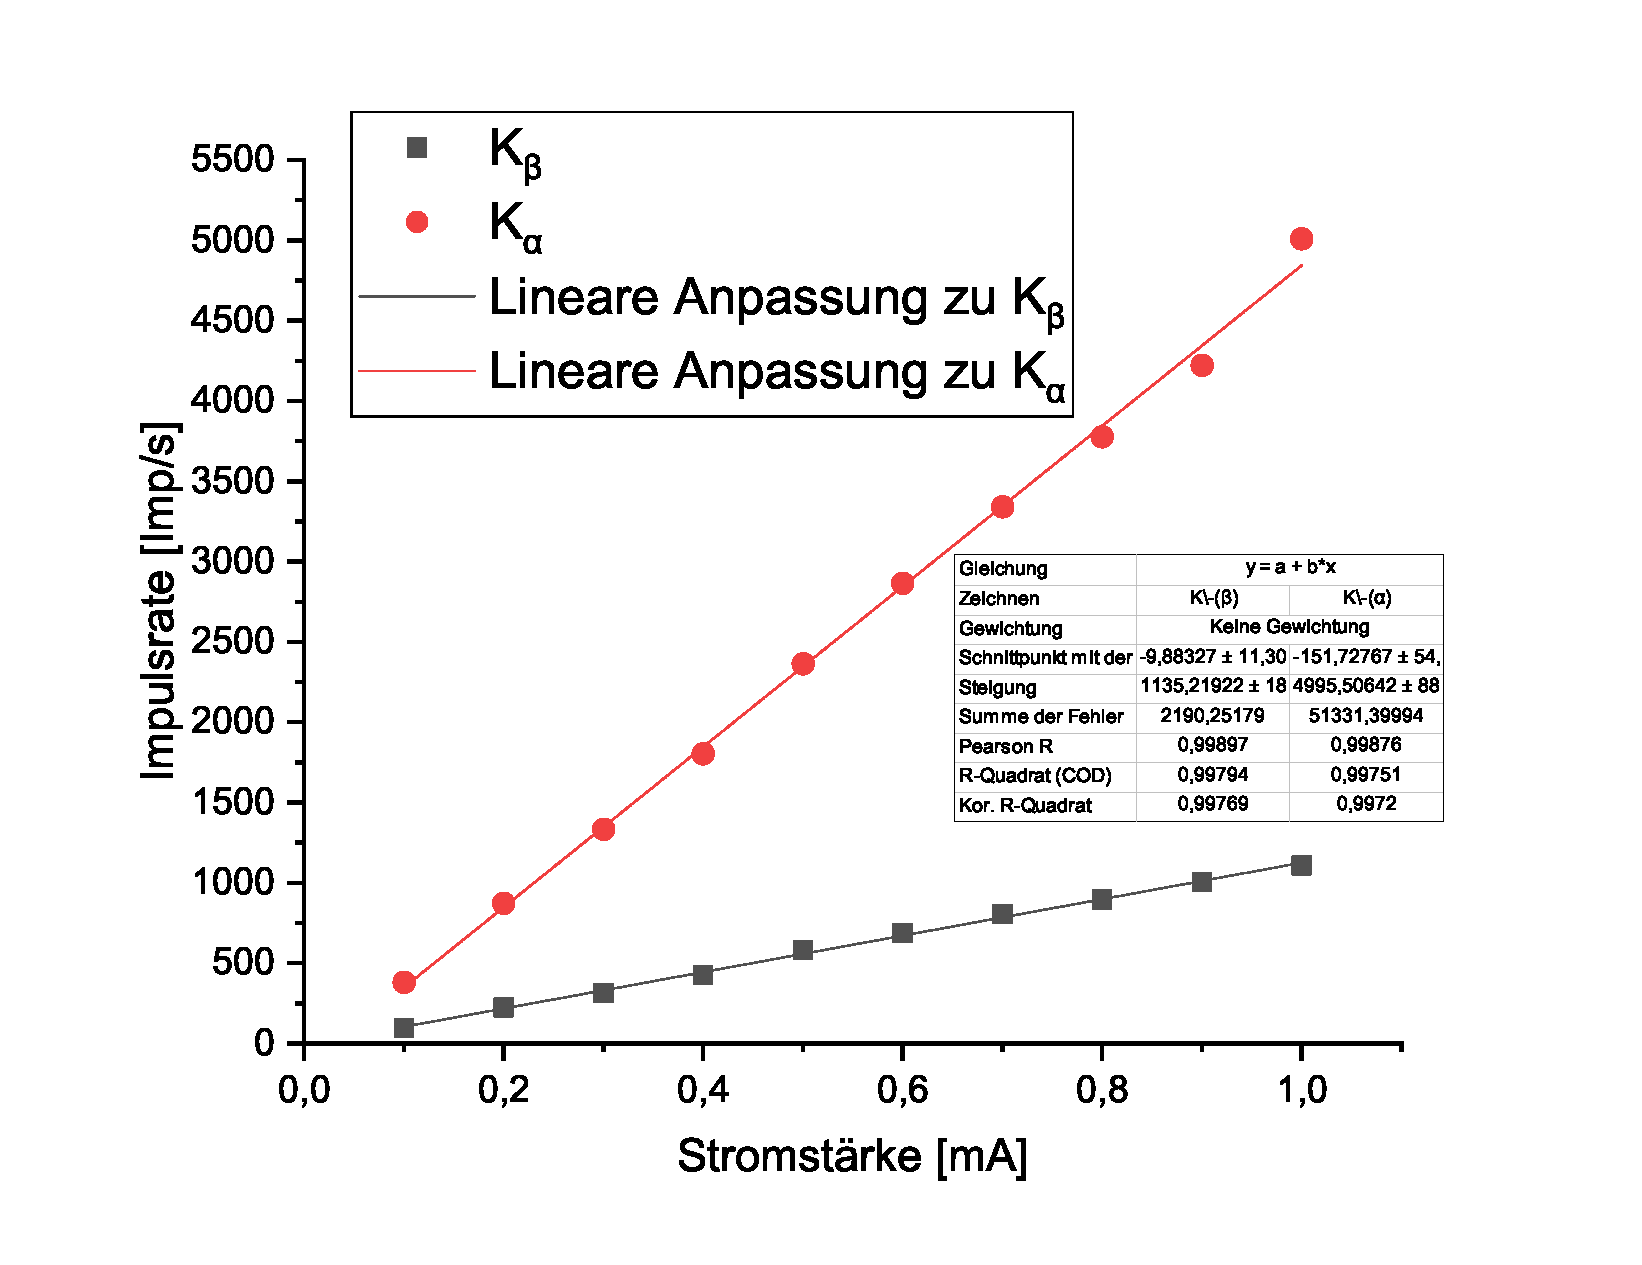
\includegraphics[scale = 0.6]{strom.eps}
	\caption{Die korrigierte Impulsrate aufgetragen gegen die angelegte Stromstärke. Der lineare Verlauf ist deutlich erkennbar.}
	\label{strom}
\end{figure}

Anschließend wurde der Einfluss einer Spannungsänderung auf die Intensität betrachtet. Auch hier entspricht die Intensität der nach \cref{eq:korr} korrigierten Impulsrate. Dieser Zusammenhang ist in \cref{spannung} dargestellt. Die Impulsrate steigt bei kleineren Spannungen erst langsam, bei höheren Spannungen aber immer stärker.

\begin{figure}[h!]
	\centering
	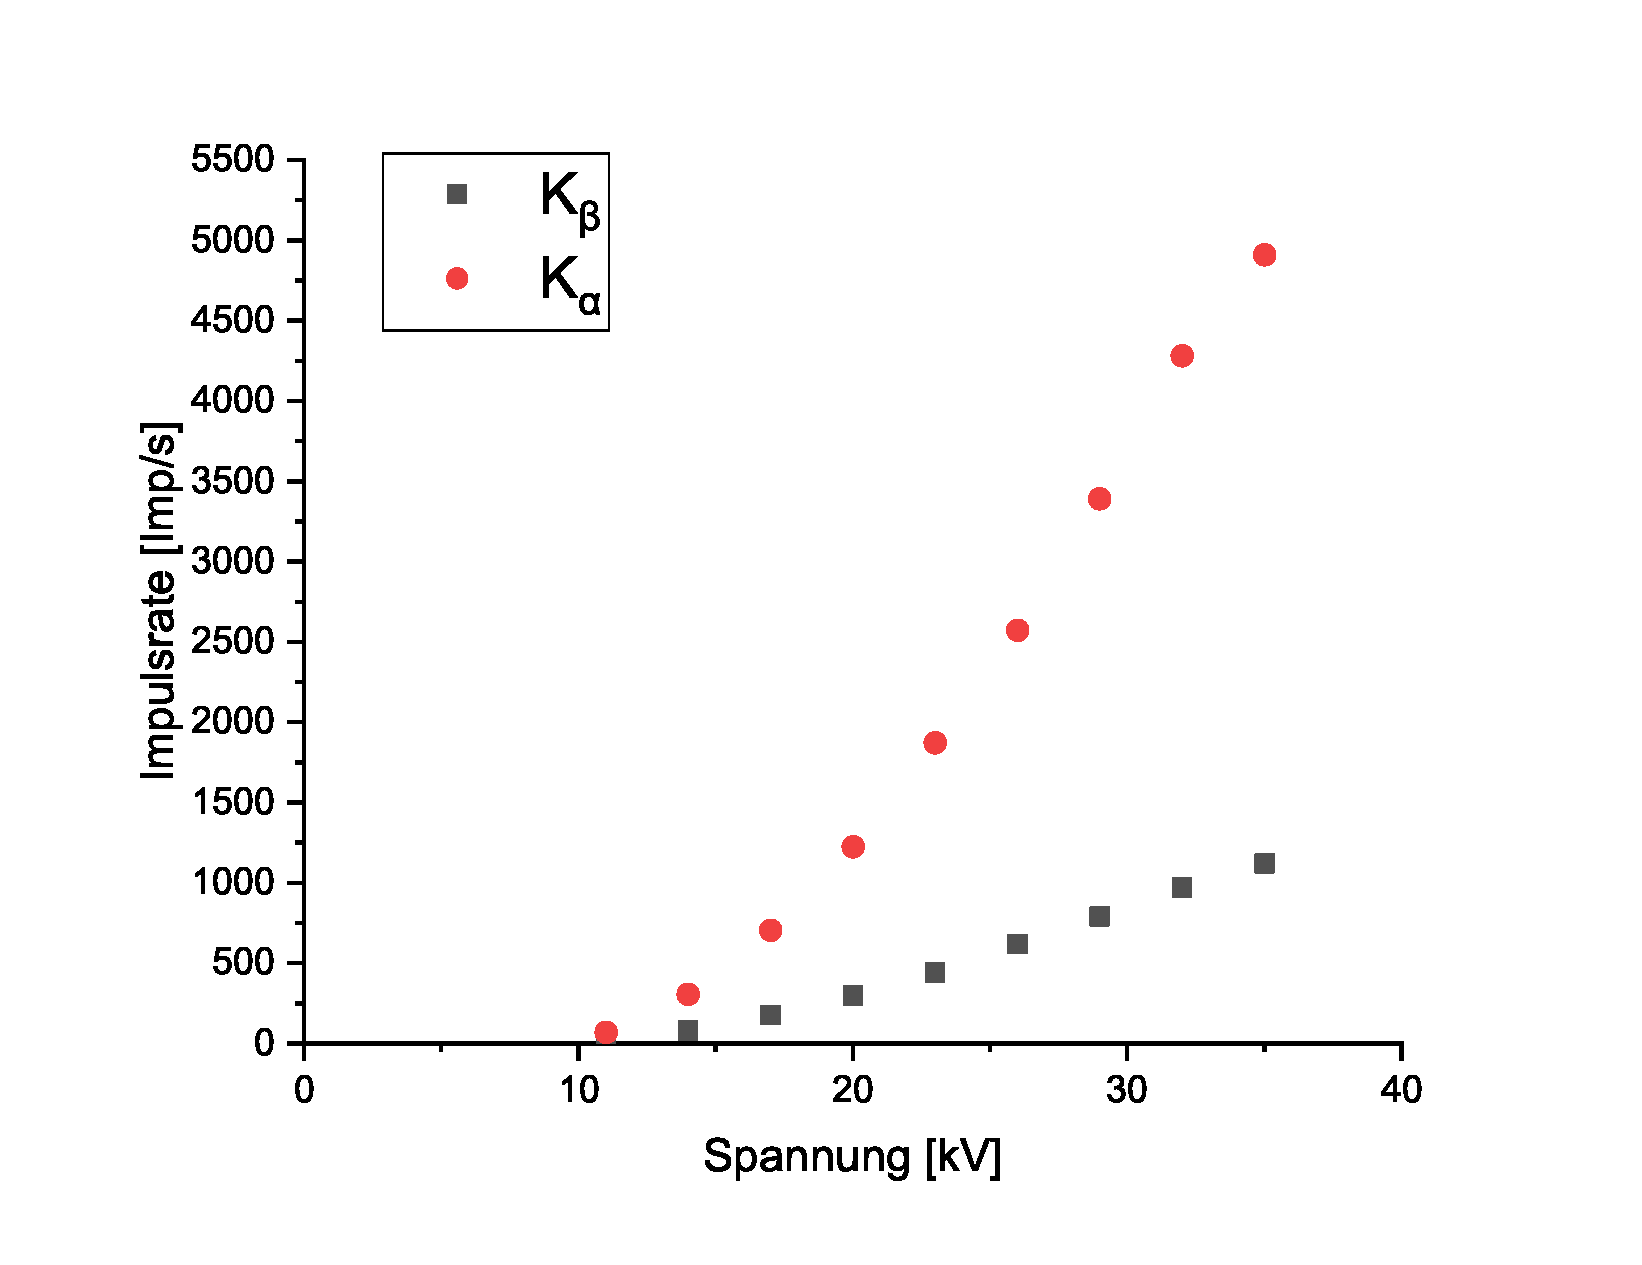
\includegraphics[scale = 0.6]{spannung.eps}
	\caption{Die korrigierte Impulsrate aufgetragen gegen die Spannung.}
	\label{spannung}
\end{figure}

 Um den in \cref{eq:ik} dargestellten Zusammenhang zu überprüfen, wurde in \cref{spannung2} die korrigierte Impulsrate gegen $(U_A - U_K)^{1,5}$ aufgetragen. Hier ist der lineare Verlauf der beiden K-Linien wieder deutlich erkennbar, so wie in \cref{eq:ik} vorhergesagt.
 
 Somit konnte in diesem Abschnitt die Gültigkeit der Formel für die K-Linien in Kupfer gezeigt werden.

\begin{figure}[h!]
	\centering
	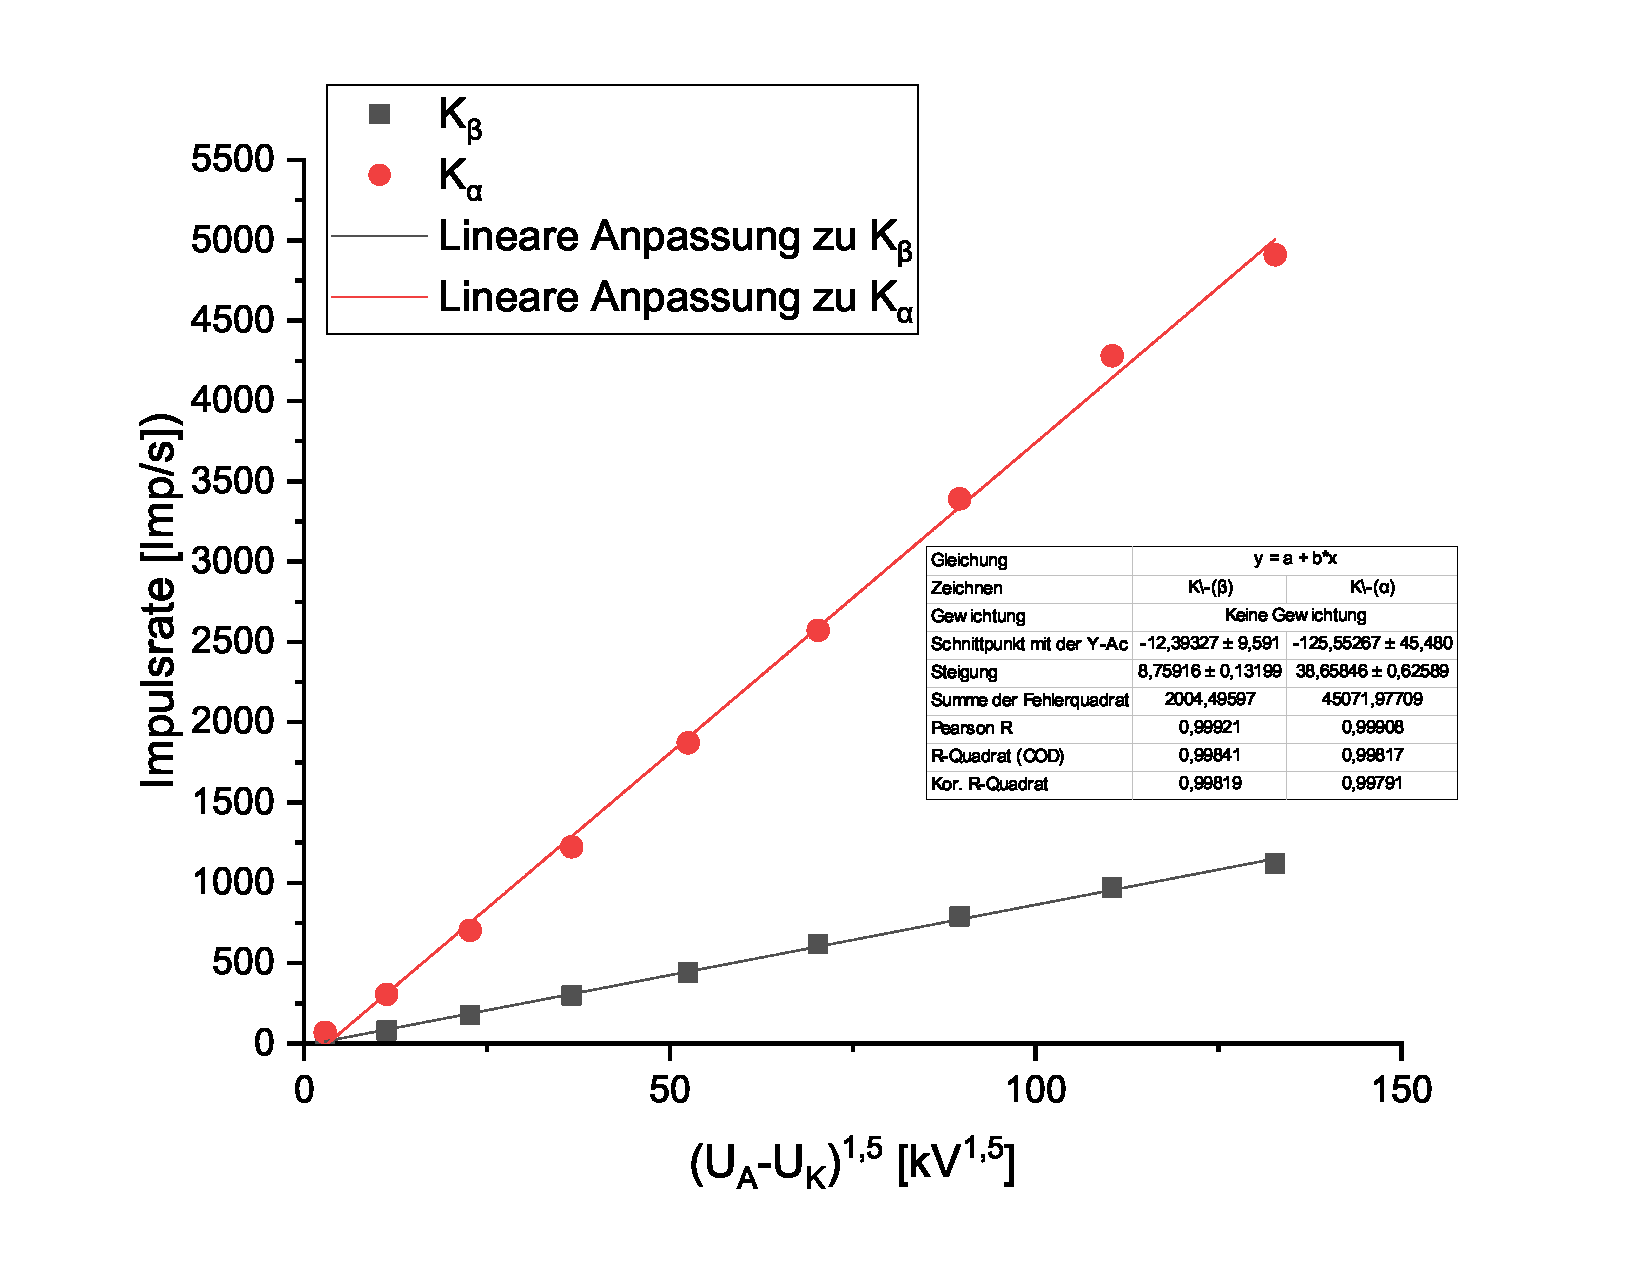
\includegraphics[scale = 0.6]{spannung2.eps}
	\caption{Die korrigierte Impulsrate aufgetragen gegen $(U_A-U_K)^{1,5}$. Der lineare Verlauf ist deutlich erkennbar.}
	\label{spannung2}
\end{figure}


\end{document}